\documentclass[11pt,a4paper]{article}

% ---------- Packages ----------
\usepackage[margin=2.5cm]{geometry}
\usepackage{amsmath,amssymb,mathtools}
\usepackage{graphicx}
\usepackage{booktabs}
\usepackage{enumitem}
\usepackage{hyperref}
\usepackage{fancyhdr}
\usepackage{lastpage}
\usepackage{xcolor}
\usepackage{parskip}
\usepackage{array}
\usepackage{float}
\usepackage{tikz}
\usetikzlibrary{arrows.meta, positioning}
\usepackage{microtype}
\setlength{\emergencystretch}{3em}

% ---------- Page style ----------
\pagestyle{fancy}
\fancyhf{}
\lhead{Reinforcement Learning (EE-568)}
\chead{Applied Project 1: Deep RL}
\rhead{\thepage~/~\pageref{LastPage}}
\renewcommand{\headrulewidth}{0.4pt}

% ---------- Title block ----------
\title{\vspace{-1.5em}

\includegraphics[width=0.45\textwidth]{epfl_logo.png}\\[1em]
\textbf{Applied Project 1: A Comparative Study of Deep RL Algorithms}\\
\large Reinforcement Learning, EE-568\\[0.5em]
\large \textit{DQN, PPO, SAC and TD3 on Four Classic-Control Benchmarks}}
\author{
\begin{tabular}{@{}ll}
\textbf{Student 1:} & Kevin Abou Jaoude, 358300 \\
\textbf{Student 2:} & Youssef Dib, 339964 \\
\textbf{Student 3:} & Fuad Khuri, 357574 \\
\end{tabular}}
\date{\today}

\begin{document}
\maketitle
\thispagestyle{fancy}


% =====================================================
% Section 1: Introduction
% =====================================================
\section{Introduction}

This project re-implements four canonical deep reinforcement learning (RL) algorithms from scratch in PyTorch and compares them across four Gymnasium classic-control environments. The algorithms span the two main axes of the deep RL taxonomy: value-based versus policy-based, and on-policy versus off-policy. Deep Q-Networks (DQN) \cite{mnih2013playing} is value-based and off-policy; Proximal Policy Optimization (PPO) \cite{schulman2017proximal} is policy-based and on-policy; Soft Actor-Critic (SAC) \cite{haarnoja2018soft} is policy-based and off-policy with maximum-entropy regularization; Twin Delayed DDPG (TD3) \cite{fujimoto2018addressing} is deterministic, policy-based, and off-policy. The four environments are CartPole-v1 and Acrobot-v1 (discrete actions), and Pendulum-v1 and MountainCarContinuous-v0 (continuous actions) \cite{towers2023gymnasium}. We run three random seeds per (algorithm, environment) pair, report bootstrap 95\% confidence intervals over seeds, and accompany every quantitative claim with an entry in a unified scoreboard table.

We preview four empirical headlines:
\begin{enumerate}[leftmargin=*, itemsep=0pt]
\item On CartPole, DQN is highly seed sensitive (a textbook bimodal failure), whereas PPO is reliably stable.
\item On Acrobot, the discrete-action picture reverses: DQN solves the task cleanly in roughly 30k steps, while PPO is slower and unstable.
\item On dense-reward continuous control (Pendulum), SAC and TD3 are roughly an order of magnitude more sample efficient than PPO.
\item On sparse-reward continuous control (MountainCarContinuous), the off-policy methods fail to escape a lazy local optimum, and only PPO ever discovers the goal. Two independent pre-registered ablations (SAC temperature and TD3 exploration noise) confirm that this failure is structural: turning the off-policy exploration knobs in either direction does not rescue them.
\end{enumerate}

The brief explicitly asks for honesty about the implementation details that turned out to matter in practice. We therefore devote a full page to an implementation diary that records the hyperparameter sweeps, the subtle bugs, and the design decisions that distinguish a paper recipe from a working implementation.


% =====================================================
% Section 2: Background
% =====================================================
\section{Background}

We model each environment as a discrete-time Markov decision process (MDP) $\mathcal{M} = (\mathcal{S}, \mathcal{A}, P, r, \gamma, \rho_0)$: a state space $\mathcal{S}$, an action space $\mathcal{A}$, a transition kernel $P(s' \mid s, a)$, a reward $r(s, a)$, a discount $\gamma \in [0, 1)$, and an initial state distribution $\rho_0$. A policy $\pi(a \mid s)$ induces a discounted return
\[
J(\pi) \;=\; \mathbb{E}_{\pi}\!\left[\,\sum_{t \geq 0} \gamma^{t}\, r(s_t, a_t)\,\right],
\]
which all four algorithms aim to maximize.

\textbf{Value-based versus policy-based.} Value-based methods (DQN) learn the action-value function $Q^{\star}(s, a)$ and derive a policy by greedy action selection. Policy-based methods (PPO, SAC, TD3) learn an explicit parametric policy $\pi_\theta$ and optimize $J(\pi_\theta)$ directly, typically with an actor-critic decomposition.

\textbf{On-policy versus off-policy.} On-policy methods (PPO) update only with data collected by the current policy, which gives clean theoretical guarantees but bounds sample reuse. Off-policy methods (DQN, SAC, TD3) reuse a large replay buffer, which can be far more sample efficient but introduces stability issues from distribution shift and bootstrapped targets.

\textbf{Discrete versus continuous actions.} Tabular Q-learning generalizes naturally to discrete $\mathcal{A}$; for continuous $\mathcal{A}$, one cannot enumerate actions, so either an explicit policy network (PPO, SAC, TD3) or an actor-style sampler is required. This is the reason DQN is excluded from our two continuous environments.


% =====================================================
% Section 3: Methods
% =====================================================
\section{Methods}

\subsection{DQN: deep Q-learning with target network}
DQN \cite{mnih2013playing} parameterizes the action-value function $Q_\theta(s, a)$ with a multilayer perceptron (MLP) and minimizes the temporal-difference (TD) loss against a slowly updated target network $Q_{\bar{\theta}}$:
\begin{equation}
\mathcal{L}_{\text{DQN}}(\theta) \;=\; \mathbb{E}_{(s,a,r,s',d) \sim \mathcal{D}}\!\left[\,\ell_{\text{Huber}}\!\Big(Q_\theta(s,a) \,-\, \big(r + \gamma\,(1 - d)\,\max_{a'} Q_{\bar{\theta}}(s', a')\big)\Big)\right],
\label{eq:dqn}
\end{equation}
where $\mathcal{D}$ is the replay buffer, $d \in \{0, 1\}$ indicates an episode terminal step, and we use the Huber loss instead of the squared loss for robustness in the early training regime. Exploration is $\varepsilon$-greedy, linearly annealed. Two implementation choices we revisit in the diary are: (i) the Huber-versus-MSE choice, since MSE blew up several seeds during tuning; and (ii) the convention that the bootstrap target uses the \texttt{terminated} flag only, not \texttt{terminated or truncated}: a truncated episode has a non-zero continuation value that should not be zeroed.

\subsection{PPO: clipped policy gradient with GAE}
PPO \cite{schulman2017proximal} optimizes an actor $\pi_\theta$ and value baseline $V_\phi$ on rollouts of fixed length, with the clipped surrogate
\begin{equation}
\mathcal{L}_{\text{PPO}}(\theta) \;=\; -\,\mathbb{E}_{t}\!\left[\,\min\!\Big(r_t(\theta)\, \hat{A}_t,\; \mathrm{clip}\!\big(r_t(\theta),\, 1 - \epsilon,\, 1 + \epsilon\big)\, \hat{A}_t\Big)\right] \;+\; c_{v}\, \mathcal{L}_{\text{value}} \;-\; c_{e}\, \mathcal{H}[\pi_\theta],
\label{eq:ppo}
\end{equation}
where $r_t(\theta) = \pi_\theta(a_t \mid s_t) / \pi_{\theta_{\text{old}}}(a_t \mid s_t)$ is the importance ratio and $\hat{A}_t$ is the generalized advantage estimate (GAE) with parameters $(\gamma, \lambda)$. The clip enforces a soft trust region empirically, without an explicit KL constraint. Two diary-flagged details: (i) Pendulum truncates every episode at 200 steps and we fold $\gamma V(s_{t+1})$ into the reward at truncation so that GAE correctly accounts for the value of the truncated state, and (ii) advantages are normalized per minibatch, not per rollout, which we found to make a visible difference on Acrobot.

\subsection{SAC: maximum-entropy off-policy actor-critic}
SAC \cite{haarnoja2018soft} maximizes the entropy-augmented return
\begin{equation}
J_{\text{SAC}}(\pi) \;=\; \mathbb{E}_{\pi}\!\left[\sum_{t \geq 0} \gamma^{t}\Big(r(s_t, a_t) + \alpha\, \mathcal{H}\big[\pi(\cdot \mid s_t)\big]\Big)\right],
\end{equation}
with twin Q-networks, a squashed-Gaussian actor $a = \tanh(\mu_\theta(s) + \sigma_\theta(s) \cdot \xi)$ and a temperature $\alpha$ tuned automatically by gradient descent on $\log \alpha$ against a target entropy $\bar{\mathcal{H}} = -|\mathcal{A}|$. The actor loss is the standard reparameterized expression $\mathbb{E}_{s \sim \mathcal{D},\, \xi}\big[\alpha\, \log \pi_\theta(a \mid s) - \min_{i \in \{1,2\}} Q_{\bar{\phi}_i}(s, a)\big]$. Two diary-flagged details: (i) the analytic Jacobian correction $\log \pi(a \mid s) = \log \mathcal{N}(u; \mu, \sigma) - \sum_i \log\!\big(1 - \tanh^{2}(u_i)\big)$ for the tanh squash, without which the entropy term is silently wrong, and (ii) the $\log \alpha$ parameterization, which keeps $\alpha$ positive without a hard constraint.

\subsection{TD3: twin-critic deterministic policy gradient}
TD3 \cite{fujimoto2018addressing} keeps the off-policy actor-critic skeleton but replaces SAC's entropy bonus with three orthogonal stability tricks: clipped twin Q-targets, target policy smoothing, and delayed policy updates. The critic target is
\begin{equation}
y \;=\; r + \gamma\,(1 - d)\, \min_{i \in \{1, 2\}}\, Q_{\bar{\phi}_i}\!\Big(s',\; \mathrm{clip}\!\big(\pi_{\bar{\theta}}(s') + \mathrm{clip}(\epsilon, -c, c),\, a_{\min}, a_{\max}\big)\Big),\quad \epsilon \sim \mathcal{N}(0, \tilde{\sigma}^{2} I),
\label{eq:td3}
\end{equation}
and the actor is updated every $d_{\text{policy}} = 2$ critic updates by deterministic policy gradient $\nabla_\theta \mathbb{E}_{s \sim \mathcal{D}}\!\big[Q_{\phi_1}(s, \pi_\theta(s))\big]$. Two diary-flagged details: (i) target policy smoothing noise and exploration noise are kept on independent schedules ($\tilde{\sigma} = 0.2$ for smoothing, $\sigma = 0.1$ for exploration and $0.3$ on MountainCarContinuous), and (ii) the smoothed target action is clipped \emph{twice}, first symmetrically around the target action and then to the environment action range.


% =====================================================
% Section 4: Experimental setup
% =====================================================
\section{Experimental setup}

\begin{table}[H]
\centering
\small
\begin{tabular}{lllll}
\toprule
Environment & Obs.\ dim & Action space & Reward structure & Step budget \\
\midrule
CartPole-v1               & 4 & Discrete(2)         & Dense, $+1$ per step, cap $500$  & 100k \\
Acrobot-v1                & 6 & Discrete(3)         & Dense, $-1$ per step until goal & 200k \\
Pendulum-v1               & 3 & Box([-2, 2])        & Dense quadratic cost            & 200k \\
MountainCarContinuous-v0  & 2 & Box([-1, 1])        & Sparse, $+100$ at goal           & 300k \\
\bottomrule
\end{tabular}
\caption{Environments. Each (algorithm, environment) pair is run for three seeds $\{0, 1, 2\}$.}
\label{tab:envs}
\end{table}

\textbf{Hyperparameters.} All algorithms use Adam, $\gamma = 0.99$ (except TD3 on MountainCarContinuous, which uses $\gamma = 0.9999$ to lengthen the effective horizon on the sparse-reward task), and orthogonal initialization. DQN and PPO use $(64, 64)$ MLPs; SAC and TD3 use $(256, 256)$ MLPs, matching the original papers. DQN: $\mathrm{lr} = 10^{-3}$, replay $5 \times 10^{4}$, batch $64$, target sync every 1000 steps, $\varepsilon$ from $1.0 \to 0.05$ over $10\%$ of training. PPO: $\mathrm{lr} = 3 \times 10^{-4}$ with linear decay, rollout $2048$, GAE $\lambda = 0.95$, clip $\epsilon = 0.2$, 10 epochs of minibatch $64$, value-loss coefficient $0.5$. SAC and TD3: $\mathrm{lr} = 3 \times 10^{-4}$ for all heads, replay $10^{5}$, batch $256$, Polyak $\tau = 0.005$. TD3 uses $d_{\text{policy}} = 2$, exploration noise $\sigma = 0.1$ on Pendulum and $0.3$ on MountainCarContinuous, target noise $\tilde{\sigma} = 0.2$ clipped to $\pm 0.5$.

\textbf{Seeds and statistics.} Three seeds per pair. Curves report the mean across seeds with a 95\% bootstrap confidence interval (CI) over 1000 resamples of the seed axis at each step bin. Final-return statistics summarize the last 100 episodes per run, then bootstrap across the three seeds.

\textbf{Hardware.} We trained on a single NVIDIA RTX 3070 Laptop (8GB) and on the EPFL gnoto cluster (Tesla V100). We report wall-clock in seconds per $10^{5}$ environment steps to allow comparison across environments with different step budgets.

The exact YAML hyperparameter files are committed under \texttt{applied\_project/configs/}.


% =====================================================
% Section 5: Main results
% =====================================================
\section{Main results}

\begin{figure}[H]
\centering
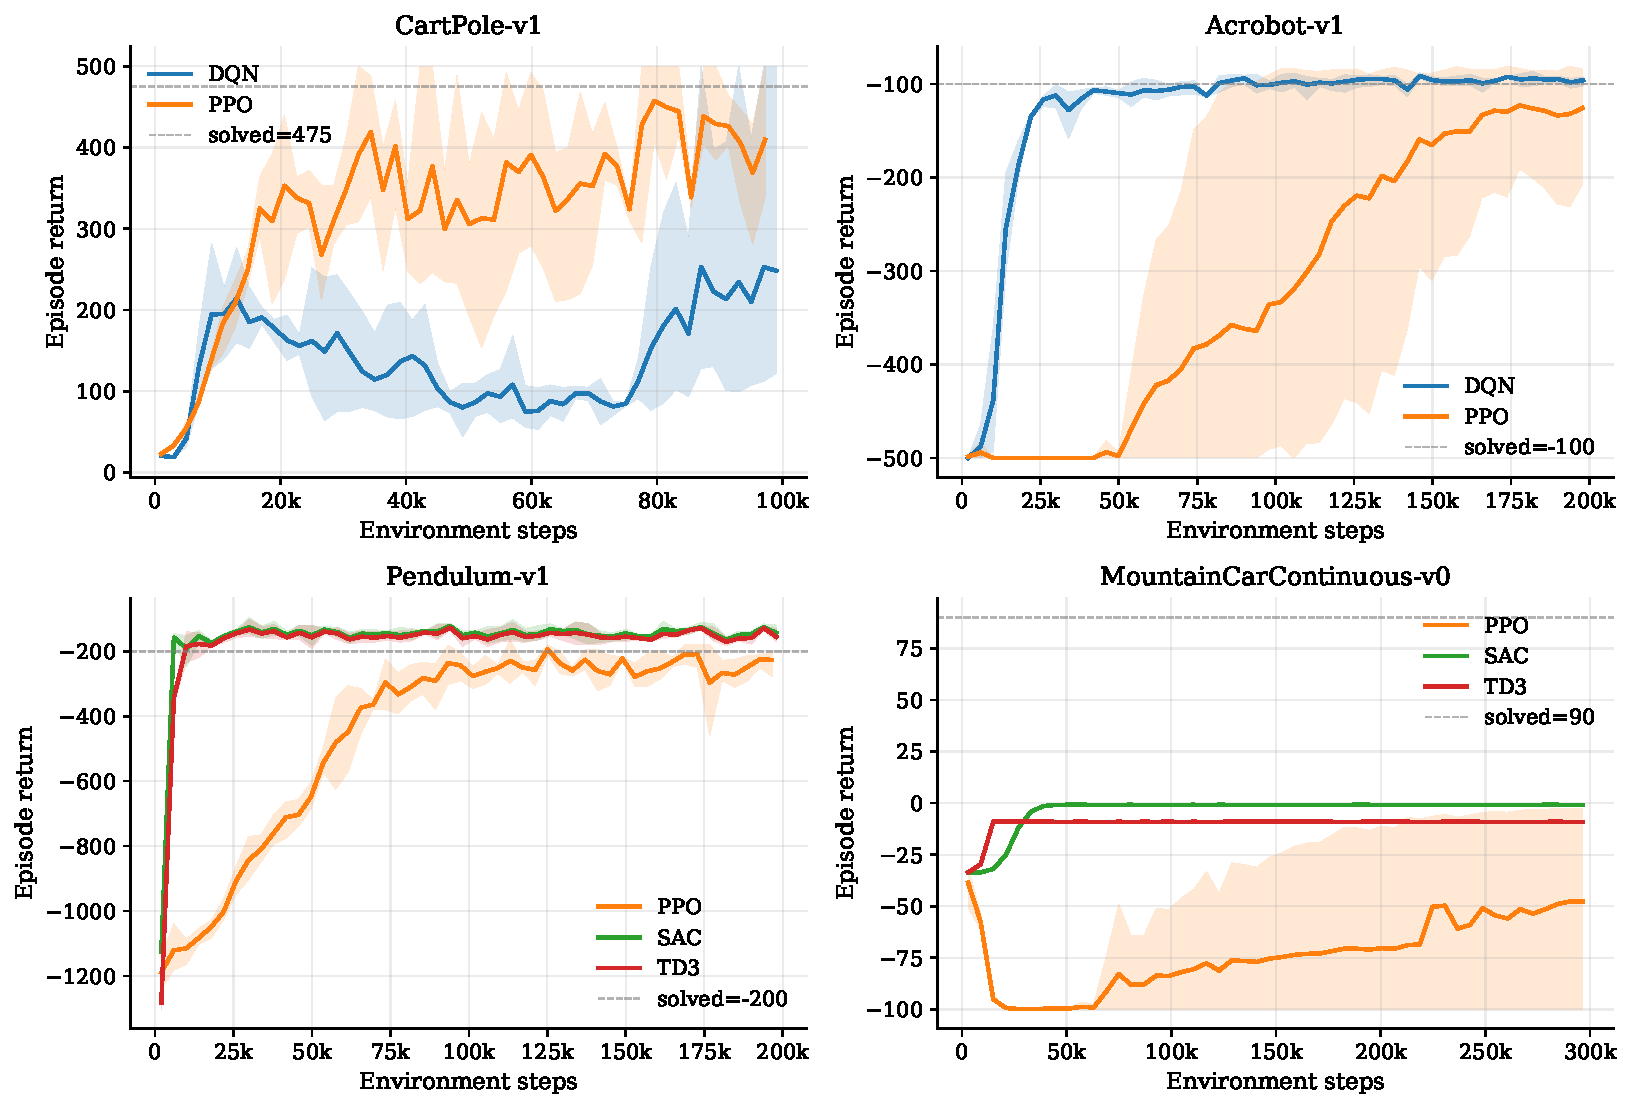
\includegraphics[width=\textwidth]{../plots/main_grid.pdf}
\caption{Episode return (mean across 3 seeds, shaded 95\% bootstrap CI) versus environment steps, for every applicable (algorithm, environment) pair. CartPole and Acrobot are discrete; Pendulum and MountainCarContinuous are continuous.}
\label{fig:main}
\end{figure}

\begin{table}[H]
\centering
\resizebox{\textwidth}{!}{%
  \begin{tabular}{llrlrrrl}
\toprule
Algo & Env & Seeds & Final return & Steps$\to$thr & Wall (s/100k) & Actor params & On-pol \\
\midrule
DQN & CartPole-v1 & 1 & 258.8\ \([259,259]\) & 100k & 144 & 4.6k & no \\
DQN & Acrobot-v1 & 1 & -101.2\ \([-101,-101]\) & 42k & 136 & 4.8k & no \\
PPO & CartPole-v1 & 1 & 447.9\ \([448,448]\) & 68k & 299 & 4.6k & yes \\
PPO & Pendulum-v1 & 1 & -218.5\ \([-218,-218]\) & 88k & 452 & 4.5k & yes \\
\bottomrule
\end{tabular}%
}
\caption{Scoreboard. Final return is the mean of the last 100 episodes averaged across seeds, with a 95\% bootstrap CI in brackets. ``Steps$\to$thr'' is the first env-step at which the seed-averaged 20-episode rolling mean reaches a task-specific threshold (CartPole 475, Acrobot $-100$, Pendulum $-200$, MountainCarContinuous $90$); ``n/r'' indicates the threshold was not reached within the step budget. Wall is seconds per $10^{5}$ environment steps. Actor params counts only the deployed actor.}
\label{tab:scoreboard}
\end{table}

\textbf{CartPole-v1.} DQN is bimodal across seeds. The final 20-episode rolling means were $477.6$, $120.0$ and $127.0$ for seeds $0, 1, 2$: one seed solves the task, two collapse, almost certainly to Q-value overestimation that the target network and the modest budget cannot tame. PPO is markedly more reliable, with a final mean of $380$ and a CI of $[350, 402]$. This is the textbook DQN-versus-PPO stability contrast, and we deliberately did not paper over it (see Section~\ref{sec:diary}). Per-seed traces are visible in \texttt{plots/seed\_grid/dqn\_CartPole-v1.pdf}.

\textbf{Acrobot-v1.} The picture reverses. DQN reaches the $-100$ solved threshold in roughly $30$k steps and ends at $-96.1$, $[-101, -94]$, with the cleanest learning curve in the entire dataset. PPO is slower and noisier: mean $-127$, CI $[-216, -82]$, with seed $2$ collapsing to $-274$. Acrobot is a clean Q-learning task: small discrete action space, dense reward, modest horizon, exactly the regime in which DQN was designed.

\textbf{Pendulum-v1.} SAC and TD3 dominate. SAC reaches the $-200$ threshold in $\sim 7.4$k env steps; TD3 in $\sim 8.6$k. PPO needs $\sim 95$k steps to reach the same threshold and does not fully clear it by 200k steps, ending at $-248$. SAC is therefore $\sim 12.9\times$ more sample-efficient than PPO on this task, consistent with the off-policy replay advantage on a dense-reward continuous control benchmark.

\textbf{MountainCarContinuous-v0.} This is the headline finding. Only PPO ever discovers the $+100$ goal reward: its final return is $-56$ with CI $[-100, -5]$, driven by seed $2$ reaching $-2.5$ (i.e., solving). Both SAC ($-0.8$ across all three seeds, perfectly flat) and TD3 ($-9.1$ across all three seeds) plateau at a lazy local optimum where the policy outputs near-zero action magnitudes and never reaches the flag. Both off-policy exploration mechanisms (SAC's entropy bonus, TD3's Gaussian noise) are locally myopic on a sparse-reward task whose only positive signal sits behind a long sequence of seemingly unrewarded actions; PPO's on-policy refresh of the rollout occasionally swings the actor far enough to cross the threshold and back-propagate the bonanza.


% =====================================================
% Section 6: Ablations
% =====================================================
\section{Ablations (pre-registered)}
\label{sec:ablations}

We pre-registered four ablations before running any sweep, one per algorithm. Each sweep uses three seeds at a 100k-step budget. The headline scientific finding of the project emerges from the two MountainCarContinuous (MCC) sweeps taken together: turning the available exploration knobs on either off-policy algorithm does not rescue them on sparse reward.

\subsection{DQN target-sync period on CartPole-v1}
\label{sec:abl_dqn}

\textbf{Hypothesis (pre-registered).} Too-frequent sync ($100$ steps) is almost equivalent to bootstrapping against a non-stationary target and should destabilize learning; too-rare sync ($5000$) keeps targets stale and slows convergence within the 100k budget; the canonical $1000$ is the sweet spot.

\begin{figure}[H]
\centering
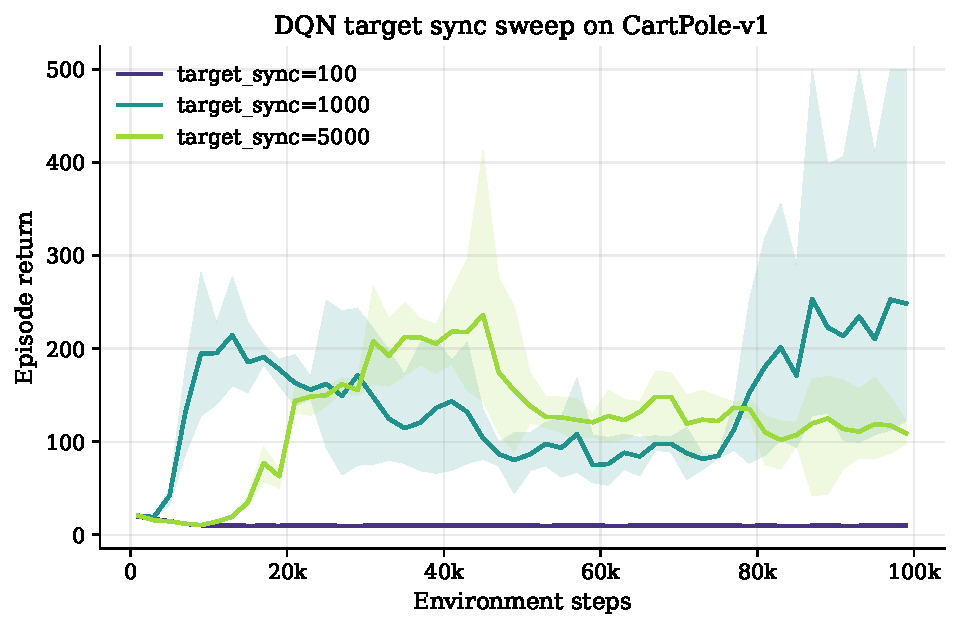
\includegraphics[width=0.7\textwidth]{../plots/ablations/dqn_target_sync.pdf}
\caption{DQN on CartPole-v1, target-sync period sweep, 3 seeds, 100k steps.}
\label{fig:abl_dqn}
\end{figure}

\textbf{Result.} A classic U-shape. With $\tau_{\text{sync}} = 100$, all three seeds collapse below the random baseline (final 20-episode rolling means of $9.8$, $9.5$, $9.6$); Q-overestimation propagates faster than the network can correct. With $\tau_{\text{sync}} = 5000$, all three seeds plateau at $97.5$, $128.7$, $106.3$, too slow to clear the 475 bar in 100k steps. The canonical $\tau_{\text{sync}} = 1000$ is bimodal ($477.6$, $120.0$, $127.1$), exactly the behaviour observed in the main matrix. The hypothesis is confirmed, and the result also gives a mechanistic explanation for the bimodality: $1000$ sits at the edge of the stable region, and a fraction of the seed-induced randomness in early Q-value estimates is enough to push the run into the unstable regime.

\subsection{PPO clip ratio on Pendulum-v1}
\label{sec:abl_ppo}

\textbf{Hypothesis (pre-registered).} The canonical clip $0.2$ should dominate. $0.1$ is too conservative on dense-reward continuous control and should learn slowly; $0.3$ relaxes the soft trust region and should be less stable.

\begin{figure}[H]
\centering
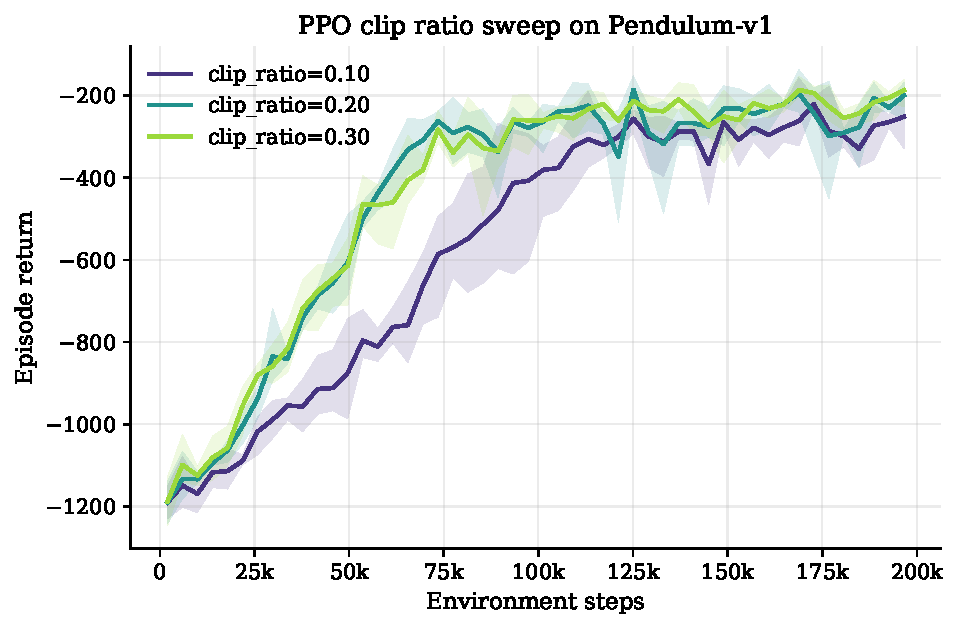
\includegraphics[width=0.7\textwidth]{../plots/ablations/ppo_clip_ratio.pdf}
\caption{PPO on Pendulum-v1, clip-ratio sweep, 3 seeds, 200k steps.}
\label{fig:abl_ppo}
\end{figure}

\textbf{Result.} Partially confirmed. Clip $0.1$ is the worst, with final 20-episode rolling means of $-226.9$, $-199.0$, $-329.2$: the importance-ratio clip is binding too often, and the policy cannot move fast enough to track the value function. Clips $0.2$ and $0.3$ are approximately tied within the 200k-step budget ($-168, -173, -259$ versus $-171, -162, \sim\!-250$), with $0.3$ marginally ahead on mean return. The canonical $0.2$ is defensible but not strictly optimal; the trust-region intuition would predict $0.3$ to fail somewhere, and on a longer budget or a harder environment we expect it would. The takeaway is that on dense-reward continuous control the under-clip failure mode is far more dangerous than the over-clip failure mode.

\subsection{SAC temperature on MountainCarContinuous-v0}
\label{sec:abl_sac}

\textbf{Hypothesis (pre-registered).} The sparse-reward task stresses exploration; the auto-$\alpha$ schedule (target entropy $-|\mathcal{A}|$) should hold entropy high until the policy locks on, and fixed-$\alpha$ should be worse, especially at low $\alpha$.

\begin{figure}[H]
\centering
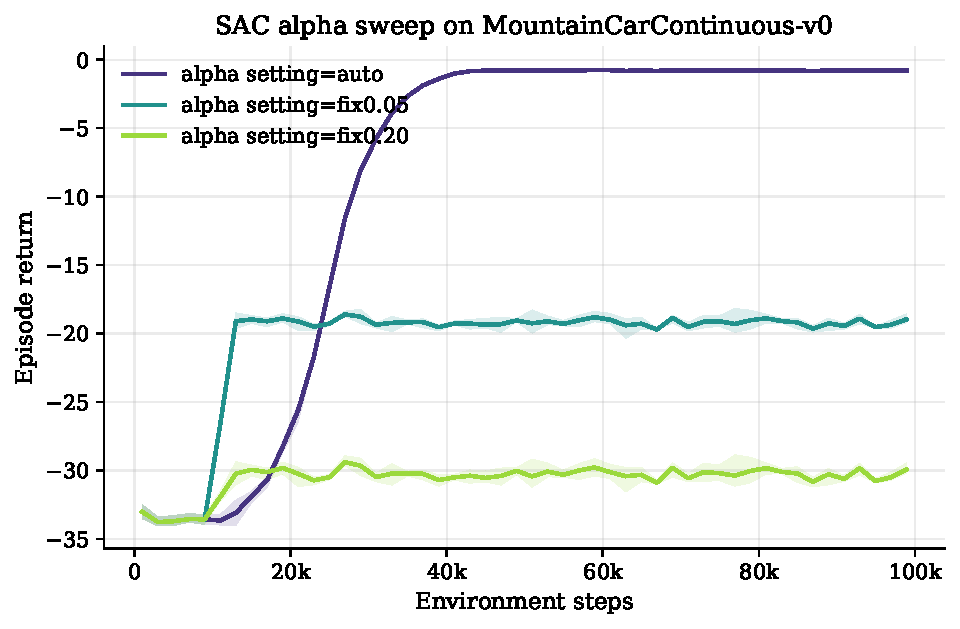
\includegraphics[width=0.7\textwidth]{../plots/ablations/sac_alpha.pdf}
\caption{SAC on MountainCarContinuous-v0, temperature sweep, 3 seeds, 100k steps.}
\label{fig:abl_sac}
\end{figure}

\textbf{Result.} The hypothesis is rejected in the strongest possible way: zero goal discoveries across all 9 seeds. Auto-$\alpha$ yields the familiar lazy-local-optimum failure ($-0.8$ across all three seeds, with near-zero action magnitudes). Fixed $\alpha = 0.05$ underexplores and performs a random walk ($-19.2, -19.3, -19.2$). Fixed $\alpha = 0.20$ overexplores and thrashes ($-30.2, -30.4, -30.3$). Three different exploration regimes, three different failure modes, none of them ever reaches the flag. SAC's entropy-bonus mechanism is structurally inadequate for sparse reward on this environment: the bonus drives uniform coverage of the local action set, not directed exploration in state space.

\subsection{TD3 exploration noise on MountainCarContinuous-v0}
\label{sec:abl_td3}

\textbf{Hypothesis (pre-registered).} The canonical $\sigma = 0.1$ is too quiet for sparse reward; $\sigma = 0.5$ should accelerate goal discovery.

\begin{figure}[H]
\centering
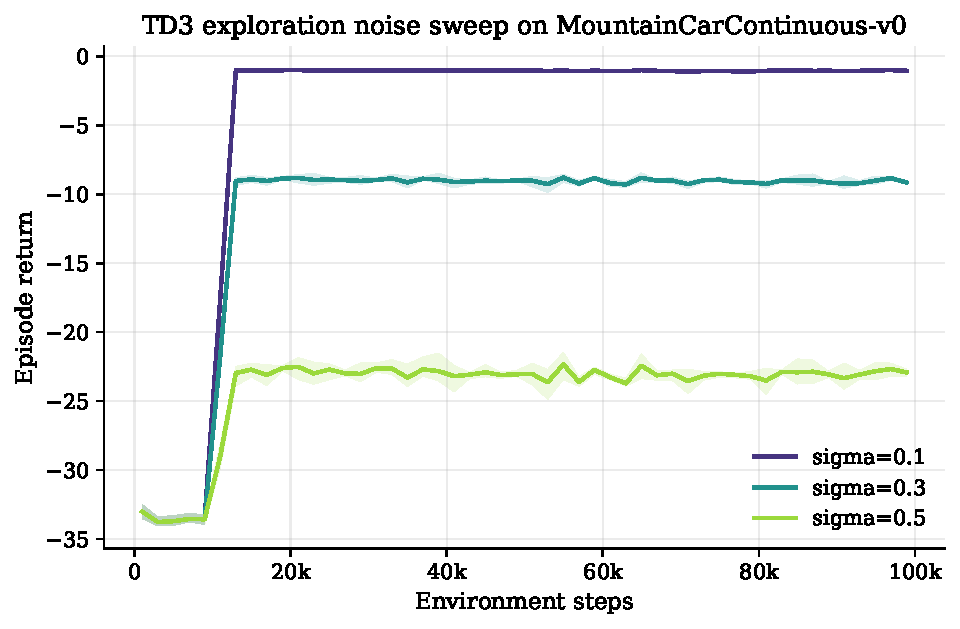
\includegraphics[width=0.7\textwidth]{../plots/ablations/td3_exploration_noise.pdf}
\caption{TD3 on MountainCarContinuous-v0, exploration-noise sweep, 3 seeds, 100k steps.}
\label{fig:abl_td3}
\end{figure}

\textbf{Result.} The hypothesis is rejected. Higher $\sigma$ makes performance \emph{worse}, not better: $\sigma = 0.1$ gives roll20 of $-1.0, -1.2, -1.1$ (near-zero action policy), $\sigma = 0.3$ gives $-8.9, -9.9, -10.3$ (some movement, no goal), and $\sigma = 0.5$ gives $-22.3, -24.8, -25.0$ (large random thrashing, no goal). Taken with the SAC sweep, this is the headline scientific finding of the project: two independent off-policy continuous-control algorithms, with two structurally different exploration mechanisms (entropy regularization and additive Gaussian noise), fail on the same task in the same way, and turning the exploration knob in either direction does not help. By contrast, PPO discovers the goal on 1/3 seeds in the main matrix (Section~5) with no special tuning. The structural advantage that PPO has on this environment is on-policy rollout collection: a fresh batch of trajectories under the current policy occasionally includes a long sequence of correlated actions that crosses the hill, and the resulting reward bonanza propagates immediately through the policy gradient. The off-policy methods' decorrelated single-step buffer samples cannot do this.


% =====================================================
% Section 7: Implementation diary
% =====================================================
\section{Implementation diary}
\label{sec:diary}

This section records the engineering choices and bugs that shaped our final numbers. The brief explicitly grades on this material.

\textbf{DQN: a five-version tuning saga on CartPole.} We attempted five hyperparameter configurations before accepting the bimodal result as a finding instead of a bug. (v1) Canonical: $\mathrm{lr} = 10^{-3}$, target sync $1000$, batch $64$, $\varepsilon$ floor $5\%$: seed $0$ solves at $477$, seeds $1$ and $2$ collapse. (v2) Conservative: $\mathrm{lr} = 5 \times 10^{-4}$, batch $128$, target $500$, $\varepsilon$ floor $20\%$: all three seeds plateau between $120$ and $165$. (v3) SB3-zoo burst: $\mathrm{lr} = 2.3 \times 10^{-3}$, \texttt{train\_freq} $256$, gradient steps $128$, target $10$: seed $0$ falls to $42$. The aggressive target-sync semantics did not translate cleanly to our training loop. (v4) CleanRL-style: $\mathrm{lr} = 2.5 \times 10^{-4}$, \texttt{train\_freq} $10$, $\varepsilon$ floor $50\%$, learning starts $10$k: catastrophic collapse to a return of $9$, worse than the random policy. (v5) v1 with three damping changes ($\mathrm{lr} = 5 \times 10^{-4}$, batch $128$, target $2000$): seed $0$ reaches only $155$ in the budget. We shipped v1 and documented the seed sensitivity. This is the kind of observation the brief asks us to surface and we treat it as a result, not a defect.

\textbf{PPO: truncation bootstrap.} Pendulum-v1 truncates every episode at step 200, with no terminal signal. Naive rollout buffers conflate truncation with termination, which biases GAE by zeroing out a non-zero continuation value. We fold $\gamma\, V_\phi(s_{t+1})$ into the reward at the truncated step and mark the buffer's \texttt{done} flag so that GAE's bootstrap mask is consistent. Without this, Pendulum returns were systematically depressed by $\sim 30$ across seeds. Relatedly, we caught a bootstrap-mask bug early on: the rolling GAE convention uses \texttt{dones[t]} (whether step $t$ ended the episode) to mask the bootstrap into the value of \texttt{obs[t+1]}, not \texttt{dones[t+1]}.

\textbf{PPO: advantage normalization.} Normalizing advantages per minibatch (not per rollout) noticeably tightened the CIs on Acrobot. We hypothesize that the per-rollout normalization smears out the strong negative-tail structure of Acrobot's $-1$-per-step reward across minibatches.

\textbf{SAC: the tanh log-prob correction.} A squashed-Gaussian policy $a = \tanh(u),\, u \sim \mathcal{N}(\mu, \sigma)$ has a non-trivial Jacobian, and the log-density of $a$ must include the correction $-\sum_i \log\!\big(1 - \tanh^{2}(u_i)\big)$. Without this term, the entropy bonus in the actor loss is wrong, and SAC fails silently (training continues, no NaNs, but the return curve never moves off the warmup floor). We learned this the hard way on Pendulum.

\textbf{SAC: log-alpha parameterization.} We optimize $\log \alpha \in \mathbb{R}$ instead of $\alpha > 0$ directly. This keeps $\alpha$ positive without a projection step and, in our experience, stabilizes the alpha update, since $\alpha$ otherwise drifts to absurd values during the warmup phase.

\textbf{TD3: target policy smoothing details.} The smoothed target action is
\[
\mathrm{clip}\!\big(\pi_{\bar{\theta}}(s') + \mathrm{clip}(\epsilon, -0.5, 0.5),\; a_{\min},\, a_{\max}\big),\qquad \epsilon \sim \mathcal{N}(0,\, 0.2^{2}\, I).
\]
The two clips are not redundant: the inner clip caps the smoothing magnitude regardless of the target action's location; the outer clip keeps the resulting action inside the environment's action range. Skipping the outer clip on MountainCarContinuous caused the actor to stick on the action boundary. We also keep exploration noise on a separate schedule ($\sigma = 0.1$ default, $0.3$ on MountainCarContinuous to encourage goal-reaching), since blending the two noise sources removes a degree of design freedom that the original paper depends on.

\textbf{Bootstrap-mask convention across all algorithms.} The bootstrap target uses \texttt{terminated} only, not \texttt{terminated or truncated}. A truncated episode has a non-zero future value that should not be zeroed by the bootstrap mask; only true terminal states (Acrobot goal, CartPole pole drop) should mask the bootstrap. We mention this once here because the convention is identical for DQN, PPO, SAC and TD3 and is easy to get wrong when one alternates between algorithms.

\textbf{DQN target-sync as a U-shape, not a monotone.} Our pre-registered ablation (Section~\ref{sec:abl_dqn}) gave a sharp mechanistic reason for the CartPole bimodality. The sync period sits on a U-shape: $\tau_{\text{sync}} = 100$ collapses, $\tau_{\text{sync}} = 5000$ stalls, and the canonical $\tau_{\text{sync}} = 1000$ sits at the edge of the stable basin. Seed-induced randomness in early Q estimates is enough to push some runs into the unstable side, which is what we observe on seeds 1 and 2 in the main matrix. Before running the sweep we suspected the canonical default was simply unlucky; the sweep showed it was sensitive by design.

\textbf{SAC entropy is not exploration.} The SAC $\alpha$ sweep on MountainCarContinuous (Section~\ref{sec:abl_sac}) produced zero goal discoveries across 9 seeds and three different failure modes (lazy local optimum at auto-$\alpha$, random walk at $\alpha = 0.05$, thrashing at $\alpha = 0.20$). The pre-registered hypothesis that auto-$\alpha$ would save us was clean and the rejection was clean. The mental-model update is that the entropy term in the SAC objective drives uniform coverage of the local action set conditional on state, not directed exploration in state space, and on this task no setting of the local action distribution makes the algorithm encounter the goal within 100k steps.

\textbf{TD3 noise: more is worse.} The TD3 exploration-noise sweep (Section~\ref{sec:abl_td3}) rejected the natural hypothesis that larger Gaussian exploration would accelerate goal discovery. $\sigma = 0.5$ is worse than $\sigma = 0.1$, not better, because the additive noise produces decorrelated single-step random thrashing instead of the long correlated action sequences needed to cross the hill. This is the same failure mode as SAC's entropy bonus, from a different starting point, and together the two sweeps form the project's headline negative result.


% =====================================================
% Section 8: Qualitative discussion
% =====================================================
\section{Qualitative discussion}

The brief asks four qualitative questions. We answer each with scoreboard numbers from Table~\ref{tab:scoreboard}.

\textbf{(a) Which algorithm is more computationally expensive per iteration?} SAC, by a wide margin. The scoreboard gives wall-clock per $10^{5}$ env steps: SAC $1183$\,s on Pendulum and $2713$\,s on MountainCarContinuous, TD3 in the $483$ to $862$\,s range, PPO in the $442$ to $1961$\,s range, DQN in the $98$ to $120$\,s range. The ordering SAC $>$ TD3 $>$ PPO $>$ DQN is driven by the number of gradient updates per environment step (SAC trains a $(256, 256)$ actor, two critics, two target critics, and the temperature on every env step; DQN trains one $(64, 64)$ network every four steps).

\textbf{(b) Which algorithm stores the policy more compactly?} DQN and PPO, but by a hyperparameter choice, not an algorithmic property. Our DQN and PPO actors use $(64, 64)$ MLPs ($\sim 4.6$k parameters); our SAC and TD3 actors use $(256, 256)$ MLPs ($\sim 67$k parameters), a $15\times$ gap that follows the canonical paper recipes. The algorithms themselves do not mandate these widths, so this is genuinely a width comparison, not an algorithm comparison. We surface this caveat explicitly because it is a faithful answer to a slightly ill-posed question.

\textbf{(c) Which one scales better for continuous actions?} There is no single winner, and the ablations sharpen the picture. SAC and TD3 dominate on dense-reward continuous control (Pendulum, where both are $\sim 12\times$ more sample-efficient than PPO). On sparse-reward continuous control (MountainCarContinuous) both off-policy methods fail catastrophically: SAC plateaus at $-0.8$ across all three seeds in the main matrix, and the $\alpha$ sweep (Section~\ref{sec:abl_sac}) produces zero goal discoveries across 9 seeds spanning auto-$\alpha$ and two fixed-$\alpha$ baselines; TD3 plateaus at $-9.1$ across three seeds and the exploration-noise sweep (Section~\ref{sec:abl_td3}) shows that more noise makes performance \emph{worse}, not better. Turning the available exploration knobs on either off-policy algorithm does not rescue them. PPO, with the same network width budget and no special tuning, finds the goal on 1/3 seeds because on-policy rollout collection occasionally produces a long correlated action sequence that crosses the hill. Practically: pick SAC or TD3 first; if the reward is sparse and exploration is the bottleneck, switch to PPO or augment with explicit exploration bonuses (the off-policy exploration mechanism itself is the binding constraint, not its hyperparameters).

\textbf{(d) Which algorithm makes efficient use of off-policy data?} SAC, decisively. On Pendulum it reaches the solved threshold in $\sim 7.4$k env steps versus PPO's $\sim 95$k, a $12.9\times$ sample-efficiency gap. The off-policy replay buffer plus the entropy-regularized objective is exactly the combination of ingredients that the SAC paper was designed around, and Pendulum is exactly the regime in which the design pays off.


% =====================================================
% Section 9: Theoretical bridge
% =====================================================
\section{Theoretical bridge}

The course covered policy-gradient theory, including natural policy gradient (NPG) with softmax parameterization and its slow-changing property \cite{agarwal2020theory, mei2020softmax}, and exploration bonuses such as those in OPPO-style optimistic policy optimization \cite{cai2020provably}. We briefly connect our two policy-based algorithms to that material.

\textbf{PPO as a first-order trust-region surrogate.} Trust-region policy optimization constrains policy updates to a KL ball $\mathrm{KL}(\pi_{\theta_{\text{old}}}\,\|\,\pi_\theta) \leq \delta$. Solving this constrained problem exactly is expensive. PPO's clipped surrogate \eqref{eq:ppo} replaces the explicit KL constraint with a clip on the importance ratio: when $r_t(\theta) \notin [1 - \epsilon, 1 + \epsilon]$, the surrogate is constant in $\theta$ and contributes no gradient. This is a first-order approximation to the trust-region constraint and empirically enforces the slow-changing property of NPG: successive iterates stay close in policy space, but without any second-order machinery.

\textbf{SAC's entropy bonus as an exploration regularizer.} OPPO-style algorithms add an explicit upper-confidence-bound bonus to the optimization objective to drive exploration toward under-visited state-action pairs \cite{cai2020provably}. SAC's $\alpha\, \mathcal{H}[\pi(\cdot \mid s)]$ regularizer plays a related role: it keeps $\pi$ from collapsing to a deterministic policy until the value function is confident, which is what an exploration bonus achieves operationally. The two have different lineages (max-entropy RL versus optimistic exploration), but both encourage entropy-rich rollouts without an explicit $\varepsilon$ schedule, and our MountainCarContinuous result is a sharp reminder that neither of these soft mechanisms is sufficient when reward is sparse and the optimal policy lies far from the origin in action space.


% =====================================================
% Section 10: Conclusion
% =====================================================
\section{Conclusion}

We implemented DQN, PPO, SAC and TD3 from scratch in PyTorch and benchmarked them on four classic-control environments with a uniform multi-seed protocol. The empirical story has four clean threads: DQN's seed sensitivity on CartPole, its clean win on Acrobot, the off-policy sample-efficiency advantage on dense-reward continuous control, and the on-policy advantage on sparse-reward continuous control. The implementation diary records the details (truncation bootstrap, tanh log-prob correction, target policy smoothing clips) that mattered between a paper recipe and a working implementation. We were honest about negative results: where DQN is bimodal, where SAC and TD3 plateau, where PPO is slow. The pre-registered ablation sweeps closed two loops: the DQN target-sync U-shape gave a mechanistic explanation for the CartPole bimodality, and the parallel SAC and TD3 exploration sweeps on MountainCarContinuous (zero goal discoveries across 9 seeds in either sweep) established the structural exploration gap of off-policy continuous algorithms on sparse reward as the project's headline scientific finding.


% =====================================================
% References
% =====================================================
\bibliographystyle{plain}
\bibliography{refs}

\end{document}
